\chapter{Literature Review\label{cha:chapter2}}

\section{Distributed Event Stores}

\section{Anonymization}

\section{Role Based Access Control}

\section{Privitar}

... should include the following:
\begin{itemize}
    \item definitions / technical terms,
    \item theoretical foundations / principles,
    \item descriptions of algorithms, hardware, software, and/or systems employed.
\end{itemize}



\begin{figure}[h]
\centering
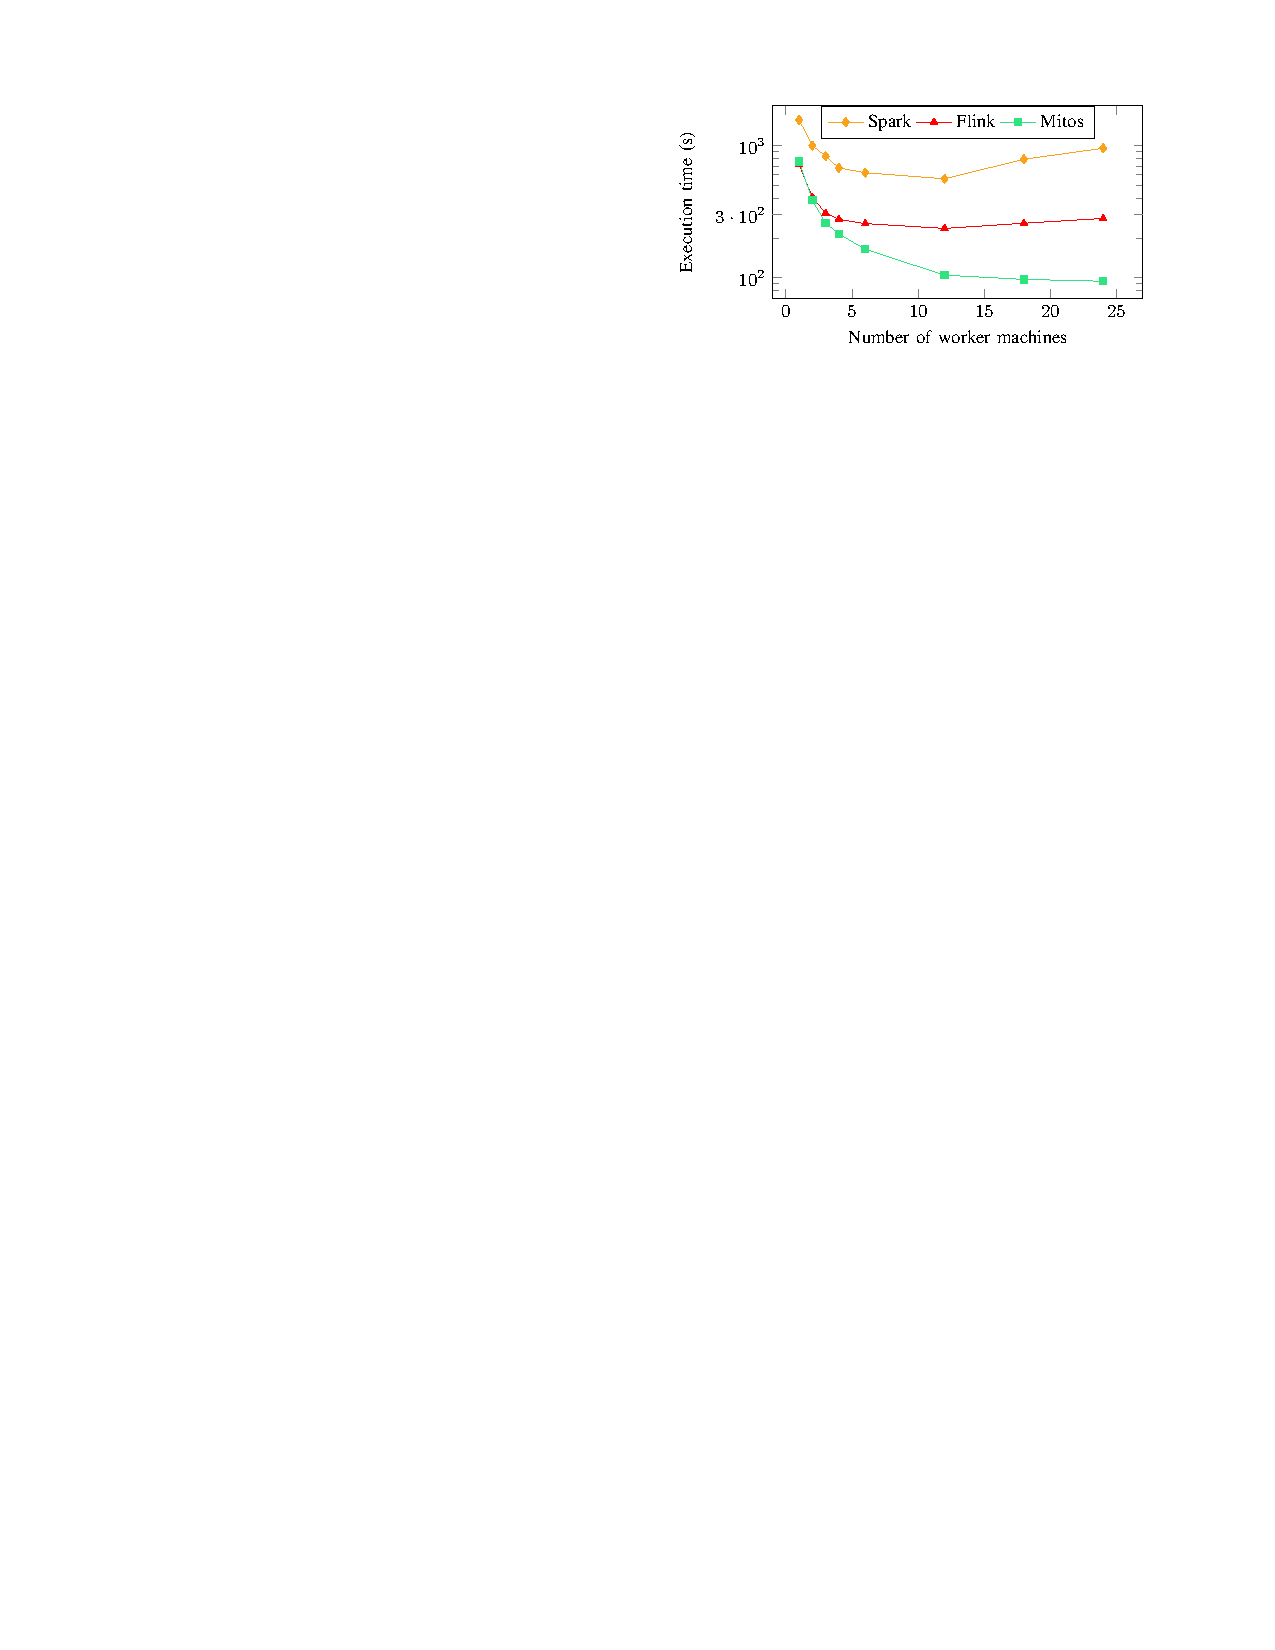
\includegraphics[width=0.6\textwidth]{./img/strong_scaling.pdf}
\caption{Strong scaling for Visit Count\cite{GevayRBMQM21}.}
\end{figure}

% We can leave this out... The advisor can point this out, if it is a concern.
%Suggestion: Figures could be inserted in pdf form to avoid pixelation when the image is magnified.

%This section is intended to give an introduction about relevant terms, technologies and standards in the field of X. You do not have to explain common technologies such as HTML or XML. 


